\documentclass{beamer}
\usepackage[utf8]{inputenc}
\usepackage{amsmath}
\usepackage{graphicx}
\usepackage{xcolor}
\usepackage{tikz}

\usetheme{Madrid}
\usecolortheme{default}

% Define custom colors inspired by Star Trek DS9
\definecolor{ds9blue}{RGB}{25,25,112}
\definecolor{ds9gold}{RGB}{218,165,32}
\definecolor{ds9grey}{RGB}{105,105,105}
\definecolor{ds9red}{RGB}{178,34,34}

% Customize the colors
\setbeamercolor{title}{fg=ds9gold}
\setbeamercolor{frametitle}{bg=ds9blue, fg=white}
\setbeamercolor{block title}{bg=ds9gold, fg=black}
\setbeamercolor{block body}{bg=ds9grey!20, fg=black}
\setbeamercolor{section in toc}{fg=ds9gold}
\setbeamercolor{subsection in toc}{fg=ds9gold!70}
\setbeamercolor{footline}{bg=ds9blue, fg=white}

\title{Further Application of Newton's Laws}
\subtitle{Friction, Drag, and Elasticity}
\author{Chapter 5}
\date{2024}

\begin{document}

\frame{\titlepage}

\begin{frame}
\frametitle{Contents}
\tableofcontents
\end{frame}

\subsection{5.1 Friction}
\begin{frame}
\frametitle{Problem 10: Snowboarder Deceleration}
\begin{block}{Problem}
Calculate the deceleration of a snow boarder going up a 5.0° slope assuming the coefficient of friction for waxed wood on wet snow is \mu_k = 0.100.
\end{block}

\begin{figure}[H]
    \centering
    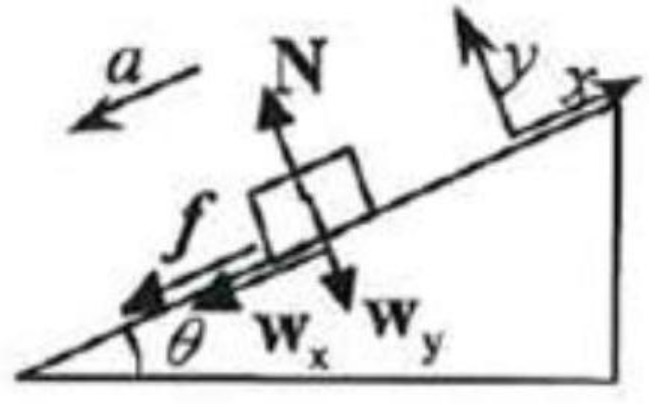
\includegraphics[width=0.5\linewidth]{CH5/Screenshot 2024-10-29 103504.png}
\end{figure}
\end{frame}

\begin{frame}
\frametitle{Problem 10: Solution Steps}
\begin{enumerate}
\item Draw the free body diagram
    \begin{itemize}
    \item Forces: Weight ($w = mg$), Normal force ($N$), Friction force ($f$)
    \end{itemize}
\item Apply Newton's Laws:
    \begin{itemize}
    \item net $F_x = w_x + f = ma$
    \item net $F_y = N - w_y = 0$
    \end{itemize}
\item Given values:
    \begin{itemize}
    \item $\theta = 5^\circ$
    \item $\mu_k = 0.100$
    \end{itemize}
\end{enumerate}
\end{frame}

\begin{frame}
\frametitle{Problem 10: Solution Steps (continued)}
\begin{enumerate}\setcounter{enumi}{3}
\item Using trigonometry:
    \begin{itemize}
    \item $w_x = w \sin \theta = mg \sin \theta$
    \item $w_y = w \cos \theta = mg \cos \theta$
    \item $f = \mu_k N = \mu_k mg \cos \theta$
    \end{itemize}
\item Solve for acceleration:
    \[a = \frac{w_x + f}{m} = \frac{mg \sin \theta + \mu_k mg \cos \theta}{m} = g(\sin \theta + \mu_k \cos \theta)\]
\item Final calculation:
    \[a = (9.80 \text{ m/s}^2)(\sin 5^\circ + (0.100)\cos 5^\circ) = 1.83 \text{ m/s}^2\]
\end{enumerate}
\end{frame}

\subsection{5.2 Drag Forces}

\begin{frame}
\frametitle{Problem 25: Rain Drop Velocity}
\begin{block}{Problem}
Calculate the velocity a spherical rain drop would achieve falling from 5.00 km:
\begin{itemize}
\item[(a)] in the absence of air drag
\item[(b)] with air drag
\end{itemize}
Given:
\begin{itemize}
\item Drop size: 4 mm
\item Density: $1.00 \times 10^3 \text{ kg/m}^3$
\item Cross-section area: $\pi r^2$
\end{itemize}
\end{block}
\end{frame}

\begin{frame}
\frametitle{Problem 25: Solution (Part a)}
Without air drag:
\begin{enumerate}
\item Use free fall equation: $v = \sqrt{2ax}$
\item Substitute values:
    \[v = \sqrt{2(9.80 \text{ m/s}^2)(5000 \text{ m})} = 313 \text{ m/s}\]
\end{enumerate}
\end{frame}

\begin{frame}
\frametitle{Problem 25: Solution (Part b)}
With air drag:
\begin{enumerate}
\item Calculate mass of raindrop:
    \begin{itemize}
    \item Volume = $\frac{4}{3}\pi r^3$
    \item $m = \rho V = 1000 \text{ kg/m}^3 \times \frac{4}{3}\pi(2 \times 10^{-3} \text{ m})^3$
    \item $m = 3.351 \times 10^{-5} \text{ kg}$
    \end{itemize}
\item Terminal velocity equation:
    \[v_t = \sqrt{\frac{2mg}{\rho CA}}\]
    where:
    \begin{itemize}
    \item $\rho = 1.21 \text{ kg/m}^3$ (air density)
    \item $C = 0.45$ (drag coefficient)
    \item $A = \pi r^2 = \pi(0.002 \text{ m})^2$
    \end{itemize}
\end{enumerate}
\end{frame}

\begin{frame}
\frametitle{Problem 25: Final Calculation}
Substituting values into terminal velocity equation:
\[v_t = \sqrt{\frac{2(3.351 \times 10^{-5} \text{ kg})(9.80 \text{ m/s}^2)}{(1.21 \text{ kg/m}^3)(0.45)\pi(0.002 \text{ m})^2}} = 9.80 \text{ m/s}\]
\end{frame}

\begin{frame}
\frametitle{Problem 30: Wrestler's Arm Bone Compression}
\begin{block}{Problem}
During a wrestling match, a 150 kg wrestler briefly stands on one hand. Calculate the shortening of the upper arm bone.
\end{block}
Given:
\begin{itemize}
\item Bone length: 38.0 cm
\item Bone radius: 2.10 cm
\item Young's modulus (bone): $9 \times 10^9 \text{ N/m}^2$
\end{itemize}
\end{frame}

\subsection{5.3 Elasticity: Stress and Strain}
\begin{frame}
\frametitle{Problem 30: Solution}
\begin{enumerate}
\item Compression equation:
    \[\Delta L = \frac{1}{Y} \frac{F}{A}L_0\]
    where:
    \begin{itemize}
    \item $Y = \text{Young's modulus} = 9 \times 10^9 \text{ N/m}^2$
    \item $F = \text{Force} = mg = (150 \text{ kg})(9.80 \text{ m/s}^2)$
    \item $A = \text{Cross-sectional area} = \pi r^2 = \pi(0.0210 \text{ m})^2$
    \item $L_0 = \text{Original length} = 0.380 \text{ m}$
    \end{itemize}
\item Final calculation:
    \[\Delta L = 4.5 \times 10^{-5} \text{ m}\]
\end{enumerate}
\end{frame}

\end{document}